\section*{Supplementary figures}

\setcounter{figure}{0}
\renewcommand{\figurename}{Figure S}
\setcounter{table}{0}
\renewcommand{\tablename}{Table S}


\begin{figure}[h]
    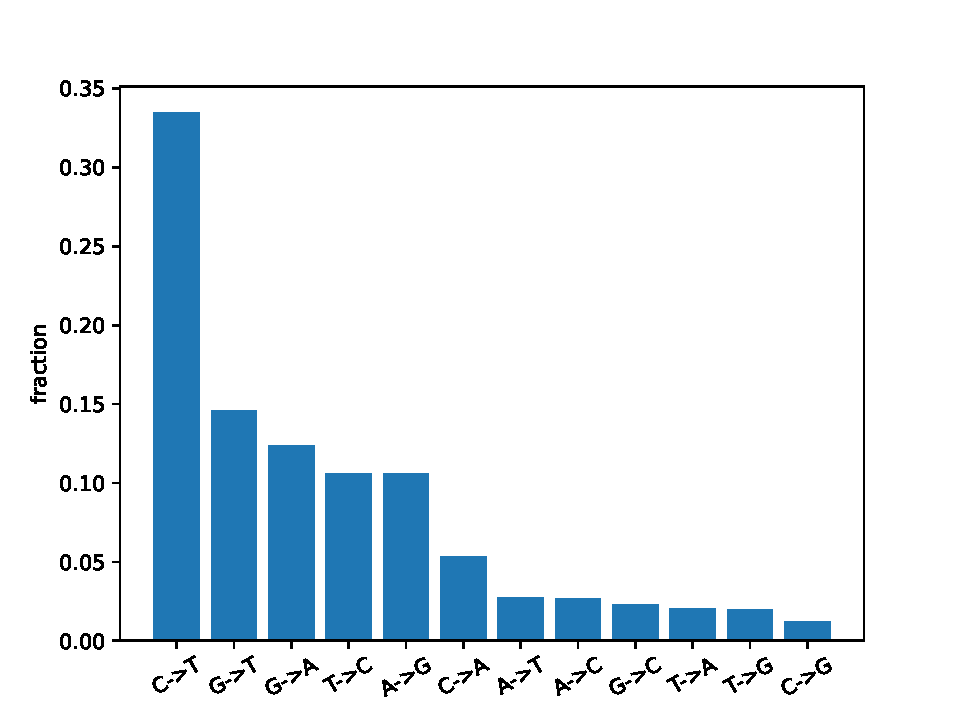
\includegraphics[width=0.5\textwidth]{figures/mutation_distribution.pdf}
    \caption{{\bf The relative rate of different mutations in SARS-CoV-2.}
    These rates are measured from rare low frequency mutations probably subject to little purifying selection.
    \label{fig:mutation_distribution}}
\end{figure}

\begin{figure}[h]
    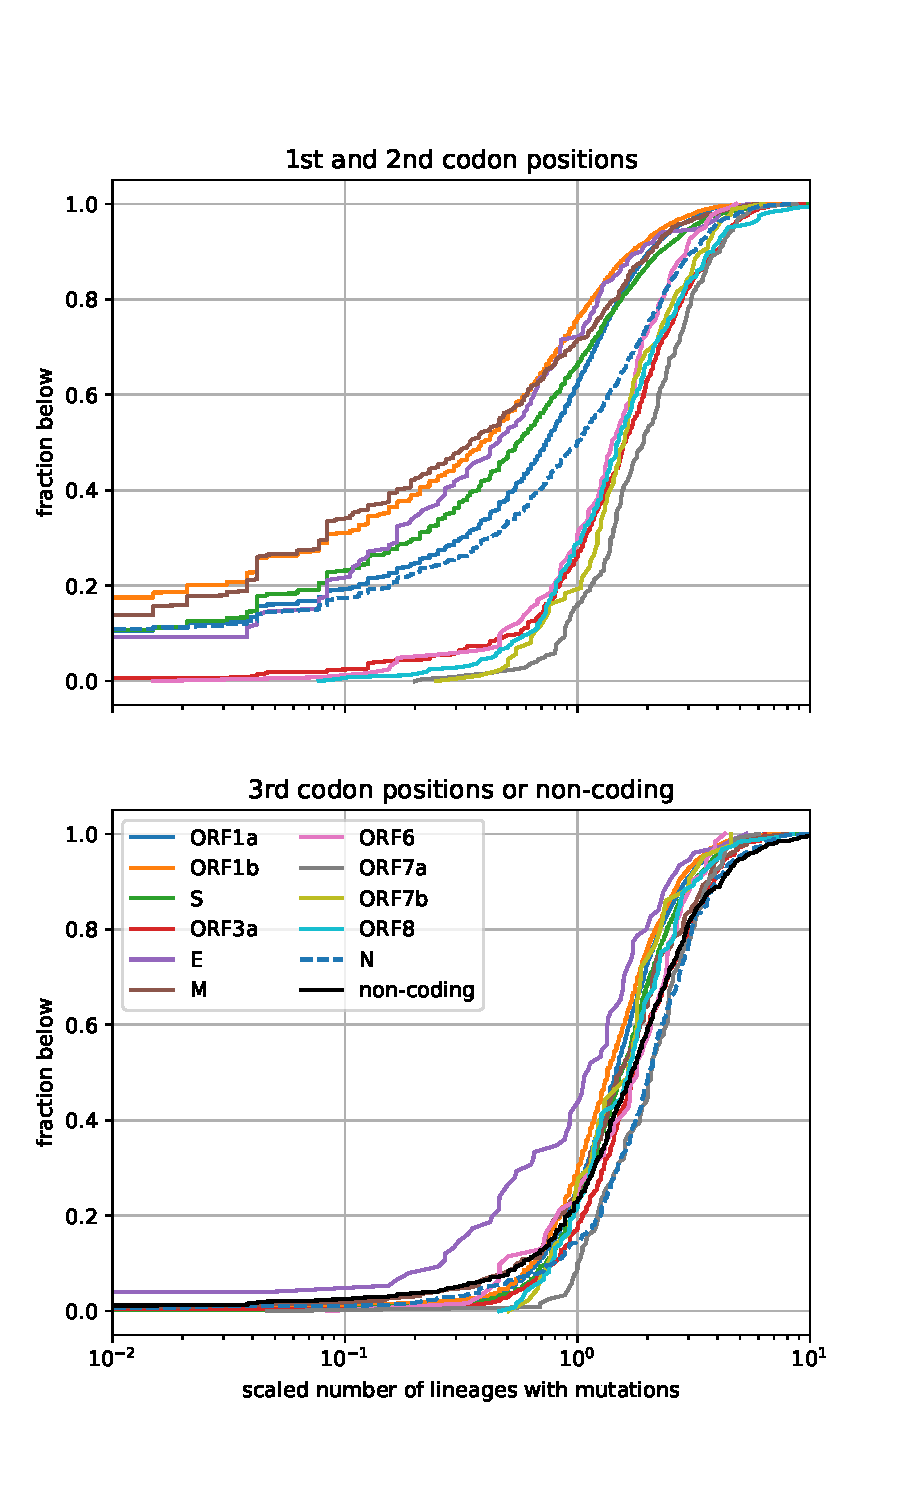
\includegraphics[width=0.5\textwidth]{figures/fitness_cost_by_gene.pdf}
    \caption{{\bf Constraints on SARS-CoV-2 mutations by gene.}
    The top panel quantifies constraint at 1st and 2nd positions in codons of open reading frames.
    The bottom panel show the analogous distributions at 3rd codon positions.
    The latter distributions are very similar across genes, with only \emph{E} showing somewhat less variation.
    In contrast, mutation tolerance at 1st and 2nd positions differs markedly between genes.
    In ORF3a, ORF6, ORF7a, ORF7b, and ORF8 the distribution of mutations at 1st and 2nd positions is very similar to the distribution at 3rd positions, while the remaining genes show clear signs of constraint.
    \label{fig:fitness_costs_supp}}
 \end{figure}
